\documentclass{beamer}
%
% Choose how your presentation looks.
%
% For more themes, color themes and font themes, see:
% http://deic.uab.es/~iblanes/beamer_gallery/index_by_theme.html
%

\mode<presentation>
{
  \usetheme{default} % or try Darmstadt, Madrid, Warsaw, ...
  \usecolortheme{default} % or try albatross, beaver, crane, ...
  \usefonttheme{serif} % or try default, structurebold, ...
  \setbeamertemplate{navigation symbols}{}
  \setbeamertemplate{caption}[numbered]
}
\newcommand*\vf[1]{\mathbf{#1}}
\usepackage[english]{babel}
\usepackage[utf8x]{inputenc}
\usepackage{amsmath,mathtools,esint,bm}
\usepackage{todonotes}
\usepackage{blindtext}
\newcommand{\mick}[1]{\textcolor{red}{[ #1 ]}}

\AtBeginSection[]{
  \begin{frame}
  \vfill
  \centering
  \begin{beamercolorbox}[sep=8pt,center,shadow=true,rounded=true]{title}
    \usebeamerfont{title}\insertsectionhead\par%
  \end{beamercolorbox}
  \vfill
  \end{frame}
}

\title[]{Charge Density Waves in Cuprates}
\author{Mick Krongchon}
\institute{University of Illinois at Urbana-Champaign}
\date{\today}

\begin{document}

\begin{frame}
\titlepage
\end{frame}

\begin{frame}{Outline}
\begin{itemize}
\item What is a phonon?
\item What is a charge density wave?
\item Summary of Miao and Dean's paper
\item My research
\item Conclusion
\end{itemize}
\end{frame}

\begin{frame}{Classical 1D chain with two masses}
\begin{itemize}
\item Each atom interacts only with its nearest neighbors
\item The system equations are
\begin{align*}
M_1 \frac{d^2}{dt^2} u_1^l = K(u_2^l - u_1^l) - K(u_1^l - u_2^{l - 1}) = K(u_2^l - 2u_1^l + u_2^{l - 1}). \\
M_2 \frac{d^2}{dt^2} u_2^l = K(u_1^{l + 1} - u_2^l) - K(u_2^l - u_1^l) = K(u_1^{l + 1} - 2u_2^l + u_1^l).
\end{align*}
\begin{figure}
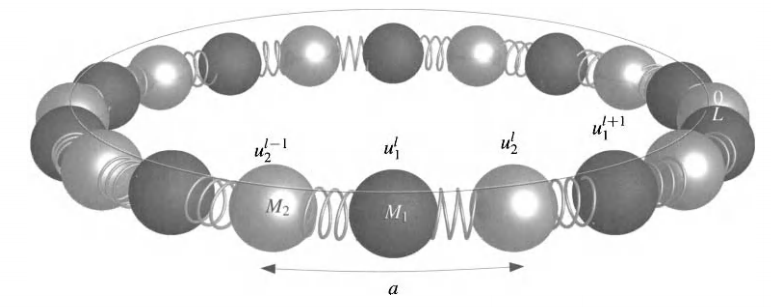
\includegraphics[width=3in]{figs/1d_diagram.png}
\caption{\label{fig:1d_diagram}} % Alternating masses $M_1$ and $M_2$ interacting with nearest neighbors
\end{figure}
\end{itemize}
\end{frame}

\begin{frame}{Phonon branches}
\begin{itemize}
\item Plug in $u_j^l = A_j e^{i(kla - \omega t)}$
\item Solve for $\omega$ that gives no trivial solutions (setting $M_2 = r M_1$):
\begin{align}
\omega = \sqrt{\frac{K}{M_1}}
\sqrt{\frac{1 + r \pm \sqrt{1 + 2r\cos{ka} + r^2}}{r}}.
\end{align}
\begin{figure}
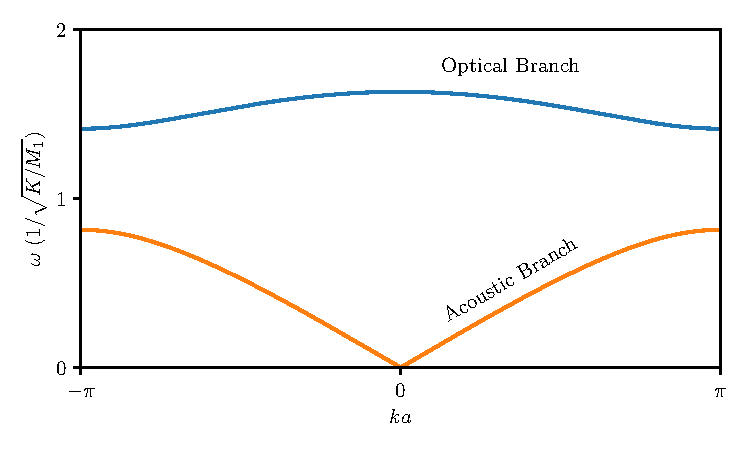
\includegraphics[width=3in]{figs/1d_dispersion.pdf}
\caption{\label{fig:1d_dispersion} $\omega(k)$ when $r = 3$}
\end{figure}
\end{itemize}
\end{frame}

\begin{frame}{Crystalline lattices are \textbf{not} 1D chains}
\begin{itemize}
% \item They are not 3D mass-spring lattices either
% \item But the idea is correct given small deviations
% \item Let $\vf{u}^1$ ... $\vf{u}^N$ describe the displacement of ions $1$ ... $N$ from their equilibrium locations $\vf{R}^1$ ... $\vf{R}^N$
\item Take the energy functional to be
\begin{align*}
\mathcal{E}(\vf{u}^1, \vf{u}^2~...~\vf{u}^N) = \mathcal{E}(u_x^1, u_y^1, u_z^1, u_x^2, u_y^2, u_z^2~...~u_x^N, u_y^N, u_z^N).
\end{align*}
\item The second-order Taylor series expansion around $\vf{O} = (\vf{0}^1, \vf{0}^2~...~\vf{0}^N)$ is
\begin{align}
\mathcal{E} &= \mathcal{E}(\vf{O}) + \sum_{\alpha,i} \frac{\partial \mathcal{E}(\vf{O})}{\partial u_\alpha^i}u_\alpha^i + \frac{1}{2} \sum_{\alpha,i} \sum_{\beta,j} \frac{\partial^2 \mathcal{E}(\vf{O})}{\partial u_\alpha^i \partial u_\beta^j} u_\alpha^i u_\beta^j, \\
&= \mathcal{E}_c + \frac{1}{2} \sum_{\alpha,i} \sum_{\beta,j} u_\alpha^i \Phi_{\alpha \beta}^{i j} u_\beta^{j}, \label{eq:3d_energy},
\end{align}
where $\alpha$ and $\beta$ range over $x$, $y$, and $z$, and $i$ and $j$ range from $1$ to $N$.
\end{itemize}
\end{frame}

% \begin{frame}{}
% \begin{itemize}
% % \item The first term is the cohesive energy, which is a constant denoted by $\mathcal{E}_c$
% \item Since the lowest energy state is a minimum as a function of ion locations, $\partial \mathcal{E}(\vf{O}) / \partial u_\alpha^i$ is zero for every $\alpha$ and $i$. The second term is zero
% % \begin{align}
% % \mathcal{E} = \mathcal{E}_c + \frac{1}{2} \sum_{\alpha,i} \sum_{\beta,j} u_\alpha^i \Phi_{\alpha \beta}^{i j} u_\beta^{j}, \label{eq:3d_energy}
% % \end{align}
% where $\Phi_{\alpha \beta}^{i j}$ is given by
% \begin{align}
% \Phi_{\alpha \beta}^{i j} = \frac{\partial^2 \mathcal{E}(\vf{O})}{\partial u_\alpha^i \partial u_\beta^j}.
% \end{align}
% \end{itemize}
% \end{frame}

\begin{frame}{}
\begin{itemize}
\item Taking the derivative to find force
\begin{align*}
F_x &=&&-\frac{\partial \mathcal{E}}{\partial u_x^l} = -\sum_i
\begin{bmatrix}
\Phi_{xx}^{li} & \Phi_{xy}^{li} & \Phi_{xz}^{li}
\end{bmatrix}
\begin{bmatrix}
u_x^i & u_y^i & u_z^i
\end{bmatrix}^\text{T}.
\end{align*}
\item Similarly for $F_y$ and $F_z$, the equation of motion is therefore
\begin{align}
\boxed{M \ddot{\vf{u}}^l = -\sum_i
\begin{bmatrix}
\Phi_{xx}^{li} & \Phi_{xy}^{li} & \Phi_{xz}^{li} \\
\Phi_{yx}^{li} & \Phi_{yy}^{li} & \Phi_{yz}^{li} \\
\Phi_{zx}^{li} & \Phi_{zy}^{li} & \Phi_{zz}^{li}
\end{bmatrix}
\begin{bmatrix}
u_x^i \\
u_y^i \\
u_z^i
\end{bmatrix} = -\sum_i \Phi^{li} \vf{u}^i}, \label{eq:phonon_motion}
\end{align}
where the subscripts are suppressed in the $3 \times 3$ matrix $\Phi^{li}$.
\item Plug in, $\vf{u}^l = \vf{A} e^{i (\vf{k} \cdot \vf{R}^l - \omega t)}$
\begin{align}
M \omega^2 \vf{A} &= \sum_{l^{\prime}} \Phi^{l l^{\prime}} e^{i \vf{k} \cdot (\vf{R}^{l^{\prime}} - \vf{R}^l)} \vf{A} = \Phi(\vf{k}) \vf{A}, \label{eq:phonon_motion_matrix}
\end{align}
\end{itemize}
\end{frame}

% \begin{frame}{}
% \begin{itemize}
% \item Plug in, $\vf{u}^l = \vf{A} e^{i (\vf{k} \cdot \vf{R}^l - \omega t)}$
% \begin{align}
% M \omega^2 \vf{A} &= \sum_{l^{\prime}} \Phi^{l l^{\prime}} e^{i \vf{k} \cdot (\vf{R}^{l^{\prime}} - \vf{R}^l)} \vf{A} = \Phi(\vf{k}) \vf{A}, \label{eq:phonon_motion_matrix}
% \end{align}
% where we replace the dummy index $i$ with $l^{\prime}$ to distinguish from the imaginary unit % , and
% % \begin{align}
% % \Phi(\vf{k}) = \sum_{l^{\prime}} e^{i \vf{k} \cdot (\vf{R}^l - \vf{R}^{l^{\prime}})} \Phi^{l l^{\prime}}. \label{eq:dyn_matrix}
% % \end{align}
% % \item Eq.~(\ref{eq:phonon_motion_matrix}) is a matrix equation for the polarization vector $\vf{A}$
% \end{itemize}
% \end{frame}

\begin{frame}{Origin of charge density waves (CDW)}
\begin{itemize}
\item The electron density in metals is uniform
\item The equilibrium positions form a perfectly periodic lattice
\item When $T < T_c$, the Fermi surface becomes unstable
\item The instability may result in periodic charge density modulation called CDW
\item In 1950s, Fr\"{o}hlich tried to explain SC that electrons and lattices move together
% \item No unifying description for CDW in different systems?
\end{itemize}
\end{frame}

\begin{frame}{Peierls' picture: 1D chain}
\begin{itemize}
% \item In 1930s, Peierls described the instability in a 1D chain of equally spaced atoms
% \item The only zero energy transition is from $k_F$ to $-k_F$, % where $k_F$ is the Fermi wave number
\item The Fermi points are at $k_F = \pm \pi / 2 a$ % connected by a vector $q = 2 k_F$
\item The disturbance with $q = 2 k_F$ changes spacing to $2 a$
\item Gap occurs at $k = \pm \pi / 2 a$
\item Metal-to-insulator transition at $T_c$ is called \textbf{Peierls' transition}
\begin{figure}
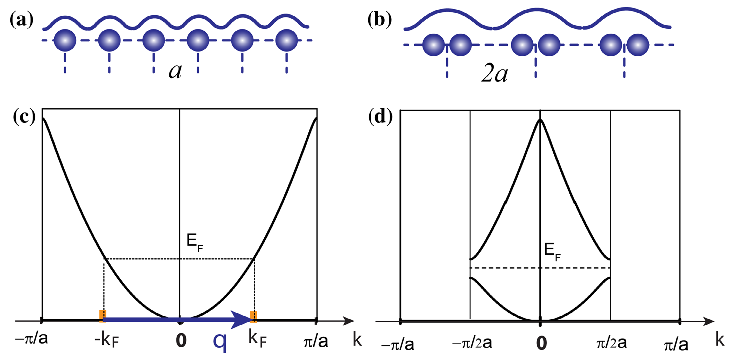
\includegraphics[width=3in]{figs/density_fermi.pdf}
\caption{\label{fig:density_fermi} (a, c) $T > T_c$ (b, d) $T < T_c$}
\end{figure}
\end{itemize}
\end{frame}

\begin{frame}{The free electron gas model}
\begin{itemize}
\item \textbf{Lindhart response function} $\chi(q)$ describes free electron gas' response
\item 1D electron gas is unstable
\begin{figure}
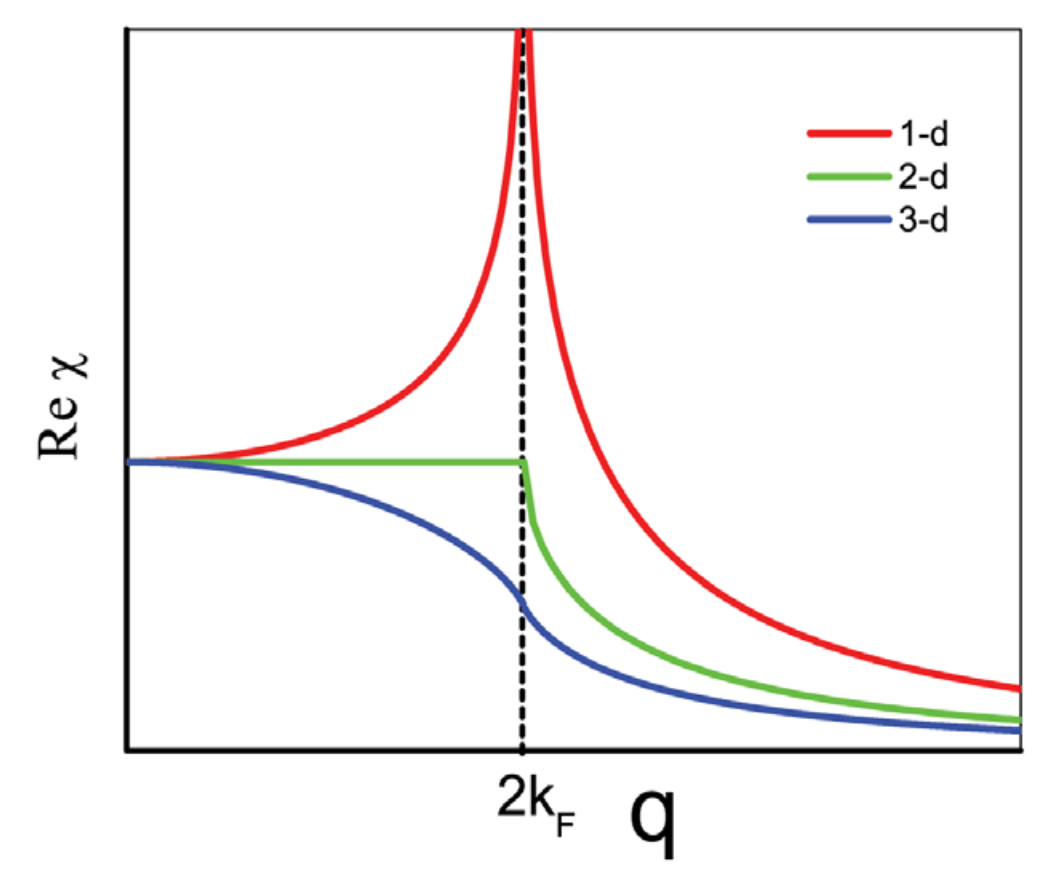
\includegraphics[width=2.5in]{figs/lindhart.png}
\caption{\label{fig:lindhart} Real part of Linhard function for 1D, 2D and 3D free electron gas models}
\end{figure}
\end{itemize}
\end{frame}

\begin{frame}{Kohn anomaly}
\begin{itemize}
\item In 1959, Kohn: The excitations at $2 k_F$ will screen any lattice motion with this wave vector
\item The phonon modes near $2 k_F$ will be renormalized to have lower energy
\item This is called \textbf{phonon softening}
%  This strong renormalization of the phonon due to interactions with an electron system is referred to as the Kohn anomaly
\begin{figure}
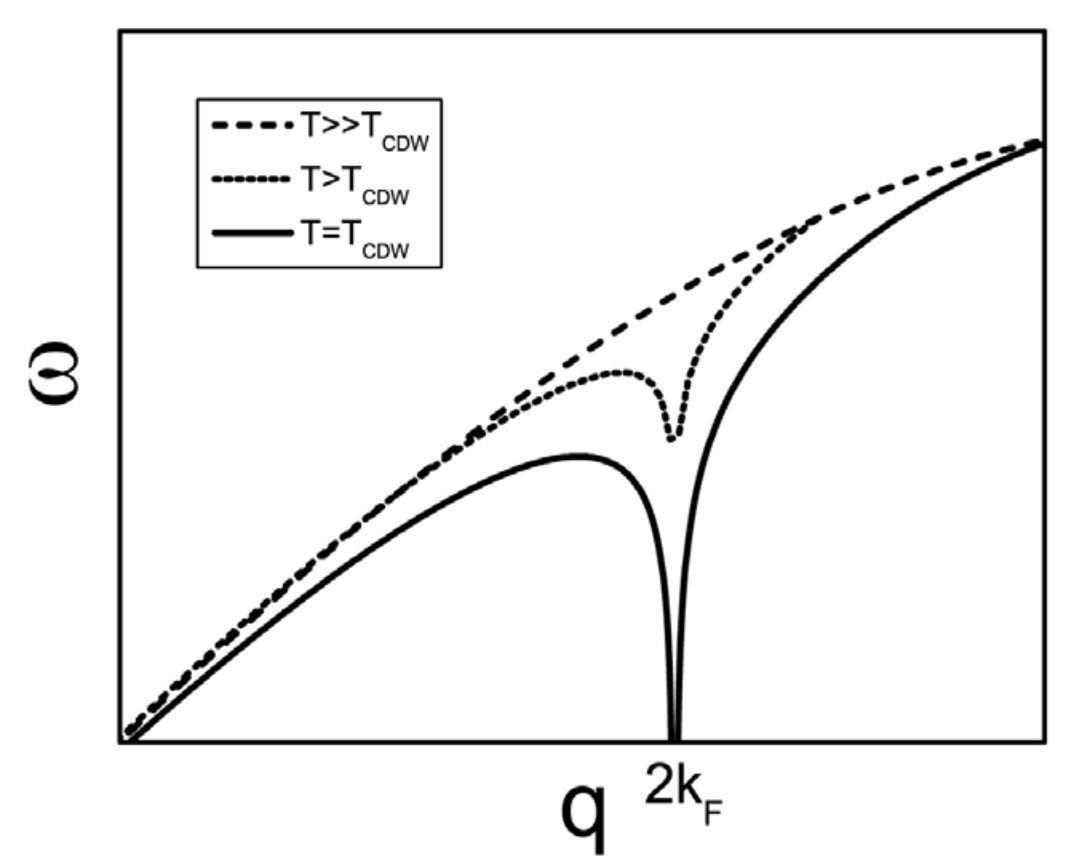
\includegraphics[width=2in]{figs/kohn_anomaly.png}
\caption{\label{fig:kohn_anomaly} Phonon energy of 1D chain at different $T$}
\end{figure}
\end{itemize}
\end{frame}

\begin{frame}{Miao and Dean's \textit{Incommensurate Phonon Anomaly and the Nature of Charge Density Waves in Cuprates (2018)}}
\begin{itemize}
\item \textit{Goal:} unifying description for superconducting cuprates
\end{itemize}
\end{frame}

% \begin{frame}{Periodic boundary conditions simplify lattice vibration calculations}
% \begin{itemize}
% \item Along any of the three primitive vectors, every physical quantity is assumed to repeat
% \item All points in the equilibrium crystal are equivalent
% \item The crystal has no surfaces or boundary
% \item Consequence: $\Phi_{\alpha \beta}^{i j}$ depends only on $\vf{R}^i - \vf{R}^j$ \mick{why?}
% \item If one displaces just two ions $\vf{u}^i$ and $\vf{u}^j$, leaving all others in equilibrium locations, the resulting energy can depend only on their relative locations
% \end{itemize}
% \end{frame}

% \begin{frame}{The dynamical equation for phonons}
% \begin{itemize}
% \item From Eq.~(\ref{eq:3d_energy}),
% \begin{align*}
% \mathcal{E} = \mathcal{E}_c + \frac{1}{2} \sum_{i = 1}^N \sum_{j = 1}^N (
% &u_x^i \Phi_{x x}^{i j} u_x^j + u_x^i \Phi_{x y}^{i j} u_y^j + u_x^i \Phi_{x z}^{i j} u_z^j + \\
% &u_y^i \Phi_{y x}^{i j} u_x^j + u_y^i \Phi_{y y}^{i j} u_y^j + u_y^i \Phi_{y z}^{i j} u_z^j + \\
% &u_z^i \Phi_{z x}^{i j} u_x^j + u_z^i \Phi_{z y}^{i j} u_y^j + u_z^i \Phi_{z z}^{i j} u_z^j).
% \end{align*}
% \item The $x$ component of the force on ion $l$ is $-\partial \mathcal{E} / \partial u_x^l$
% \item We split the sum into three parts: 1) $j = j = l$, 2) $i \neq l$ and $j = l$, and 3) $i = l$ and $j \neq l$
% \end{itemize}
% \end{frame}

% \begin{frame}{}
% \begin{itemize}
% \item Dropping the terms without $u_x^l$ because they give zero contributions to the derivative, we get
% \begin{align*}
% \frac{\partial \mathcal{E}}{\partial u_x^l}
% &=&&\frac{1}{2} \frac{\partial}{\partial u_x^l} (u_x^l \Phi_{xx}^{ll}u_x^l + 2 u_x^l \Phi_{xy}^{ll} u_y^l + 2 u_x^l \Phi_{xz}^{ll} u_z^l) + \\
% & &&\frac{1}{2}\frac{\partial}{\partial u_x^l} \sum_{i \neq l} (u_x^i \Phi_{xx}^{il} u_x^l + u_y^i \Phi_{yx}^{il} u_x^l + u_z^i \Phi_{zx}^{il} u_x^l) + \\
% & &&\frac{1}{2}\frac{\partial}{\partial u_x^l} \sum_{j \neq l} (u_x^l \Phi_{xx}^{lj} u_x^j + u_x^l \Phi_{xy}^{lj} u_y^j + u_x^l \Phi_{xx}^{lj} u_x^j) \\
% &=&&\frac{1}{2}(2 \Phi_{xx}^{ll} u_x^l + 2 \Phi_{xy}^{ll} u_y^l + 2 \Phi_{xz}^{ll} u_z^l) + \\
% & &&\frac{1}{2}\sum_{i \neq l}(u_x^i \Phi_{xx}^{il} + u_y^i \Phi_{yx}^{il} + u_z^i \Phi_{zx}^{il}) + \\
% & &&\frac{1}{2}\sum_{j \neq l}(\Phi_{xx}^{lj} u_x^j + \Phi_{xy}^{lj} u_y^j + \Phi_{xz}^{lj} u_z^j).
% \end{align*}
% \end{itemize}
% \end{frame}


% \begin{frame}{}
% \begin{itemize}
% \item The matrix $\Phi(\vf{k})$ is real and symmetric, and therefore has three orthogonal eigenvectors for every $k$
% \item Let $\vf{A}_{\vf{k} 1}$, $\vf{A}_{\vf{k} 2}$, and $\vf{A}_{\vf{k} 3}$ be eigenvectors of $\Phi(\vf{k})$, which correspond to eigenvalues $\Phi_1$, $\Phi_2$, and $\Phi_3$
% \item Eq.~(\ref{eq:phonon_motion_matrix}) gives
% \begin{align}
% \omega_{\vf{k} \nu}^2 = \frac{\Phi_\nu(\vf{k})}{M},~\nu = 1, 2, 3.
% \end{align}
% \item The three polarization vectors $\vf{A}_{\vf{k} \nu}$ comprise one longitudinal mode where $\vf{A}$ points along $\vf{k}$, and two transverse modes where $\vf{A}$ is perpendicular to $\vf{k}$
% \end{itemize}
% \end{frame}

% \begin{frame}{$\Phi^{l l^{\prime}}$ must obey some important symmetries}
% \begin{itemize}
% \item The energy of the crystal cannot change if all ions are simultaneously displaced by a single vector. Thus,
% \begin{align}
% \sum_{l^{\prime}} \Phi^{l l^{\prime}} = 0_{3,3}. \mick{\text{why?}}
% \end{align}
% From Eq.~(\ref{eq:dyn_matrix}), we have
% \begin{align}
% \Phi(\vf{k} = \vf{0}) = 0_{3,3}.
% \end{align}
% \item Applying periodic boundary conditions to Eq.~(\ref{eq:phonon_motion_matrix}) gives
% \begin{align}
% \Phi(\vf{k} + \vf{K}) = \Phi(\vf{k}),
% \end{align}
% where $\vf{K}$ is any reciprocal lattice vector.
% \end{itemize}
% \end{frame}

% \begin{frame}{Lattice with a basis leads to more than one branch}
% \begin{itemize}
% \item The same phenomenon persists in 3D
% \item Adding new atoms to a unit cell adds new degrees of freedom to the lattice
% \item One must consider a correspondingly greater number of normal modes to describe them
% \item For example, in three dimensions with four atoms per unit cell, one has $3 \times 4$ normal modes for every value of $\vf{k}$
% \item The equation of motion is now
% \begin{align}
% M_n \ddot{\vf{u}}^{l n} = -\sum_{l^{\prime} n^{\prime}} \Phi^{l n l^{\prime} n^{\prime}} \vf{u}^{l^{\prime} n^{\prime}},
% \end{align}
% where the superscripts $n$ and $n^{\prime}$ label the different atoms comprising the basis in each unit cell.
% \end{itemize}
% \end{frame}

% \begin{frame}
% \begin{itemize}
% \item Following the same procedure, the solution is taken to be
% \begin{align}
% \vf{u}^{l n} = \vf{A}^n e^{i \vf{k} \cdot \vf{R}^{l n} - i \omega t},
% \end{align}
% which leads to
% \begin{align}
% M_n \omega^2 \vf{A}^n = \sum_{n^{\prime}} \Phi^{n n^{\prime}}(\vf{k}) \vf{A}^{n^{\prime}}.
% \end{align}
% \item To simplify the problem, we define a new index $p$ that ranges over all degrees of freedom in the unit cell
% \item With four atoms per unit cell, $p$ would range from 1 to 12
% \item Using this notation,
% \begin{align}
% M_p \omega^2 A_p = \sum_{p^{\prime}}^{3N} \Phi_{p p^{\prime}} (\vf{k}) A_{p^{\prime}}.
% \end{align}
% \end{itemize}
% \end{frame}

% \begin{frame}{Example: diamond lattice}
% \begin{itemize}
% \item Suppose one has a collection of atoms sitting on a Bravais lattice $\vf{R}^{l}$ with basis $\vf{v}^n$
% \item Take $\vf{R}^{l n} = \vf{R}^l + v^n$, and have particles interact with a potential of the form
% \begin{align}
% U = \frac{1}{2} \sum_{l n l^{\prime} n^{\prime}} \phi_{n n^{\prime}} (|\vf{u}^{ln} + \vf{R}^{ln} - \vf{u}^{l^{\prime} n^{\prime}} - \vf{R}^{l^{\prime} n^{\prime}}|) \mick{\text{What sum exactly?}}.
% \end{align}
% Expanding to quadratic order in the small deviations $\vf{u}$ and using the fact that terms linear in $\vf{u}$ must vanish, we find
% \begin{align}
% U \approx \frac{1}{4} \sum_{l n l^{\prime} n^{\prime}} (\vf{})
% \end{align}
% \end{itemize}
% \end{frame}

\end{document}
